\section{Conditional Partial Order Graphs\label{sec:CPOG-model-essentials}}

A \emph{Conditional Partial Order Graph}~\cite{2009_mokhov_phd}\cite{2010_mokhov_ieee}
is a quintuple $H=(V,\ E,\ X,\ \rho,\ \phi)$, where $V$ is a finite
set of \emph{vertices}, $E\subseteq V\times V$ is a set of \emph{arcs}
between them, and $X$ is a finite set of \emph{operational}\emph{variables}. An \emph{opcode} is an assignment $(x_{1},\ x_{2},\ \dots,\ x_{|X|})\in\{0,\ 1\}^{|X|}$
of these variables; $X$ can be assigned only those opcodes which
satisfy the \emph{restriction function} $\rho$
of the graph, i.e. $\rho(x_{1},\ x_{2},\ \dots,\ x_{|X|})=1$. Function
$\phi$ assigns a Boolean \emph{condition} $\phi(z)$ to every vertex
and arc $z\in V\cup E$ of the graph.

\begin{figure}[h]
\hfill{}\subfloat[Full notation]{

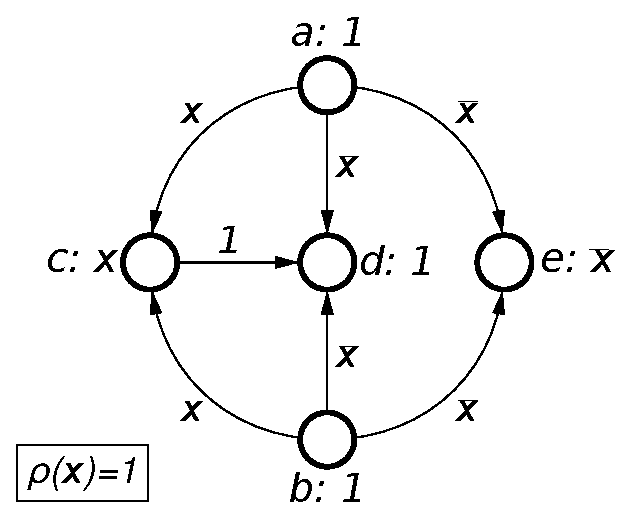
\includegraphics[scale=0.45]{fig/cpog}}\hfill{}\subfloat[Simplified notation]{

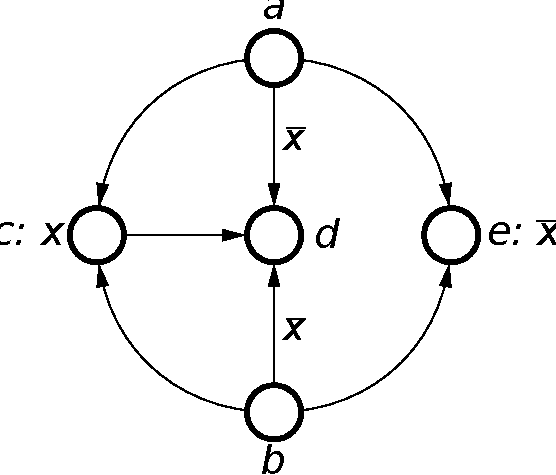
\includegraphics[scale=0.45]{fig/cpog_simplified}}\hfill{}

\begin{centering}
\subfloat[Multiple CPOG projections]{\begin{centering}
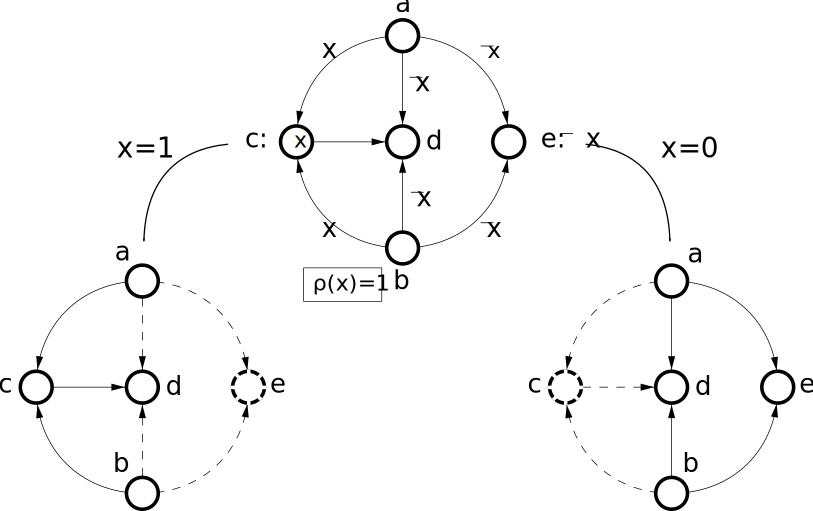
\includegraphics[scale=0.45]{fig/cpog_projections_2}
\par\end{centering}

}
\par\end{centering}

\caption{\label{fig-cpog-examples}Graphical representation of CPOGs and their projections}
\end{figure}


Figure~\ref{fig-cpog-examples}(a) shows an example of a CPOG containing
$|V|=5$ vertices and $|E|=7$ arcs. There is a single operational
variable $x$; the restriction function is $\rho(x)=1$, hence both
opcodes $x=0$ and $x=1$ are allowed. Vertices $\{a,\ b,\ d\}$ have
constant $\phi=1$ conditions and are called \emph{unconditional},
while vertices $\{c,\ e\}$ are \emph{conditional} and have conditions
$\phi(c)=x$ and $\phi(e)=\overline{x}$ respectively. Arcs also fall
into two classes: unconditional (arc $c\rightarrow d$) and conditional
(all the rest). As CPOGs tend to have many unconditional vertices
and arcs we use a simplified notation in which conditions equal to
$1$ are not depicted in the graph. This is demonstrated in Figure~\ref{fig-cpog-examples}(b).

The purpose of conditions $\phi$ is to `switch off' some vertices
and/or arcs in the graph according to the given opcode. This makes
CPOGs capable of specifying multiple partial orders or instructions
(a partial order is a form of behavioural description of an instruction).
Figure~\ref{fig-cpog-examples}(c) shows a graph and its two \emph{projections}.
The leftmost projection is obtained by keeping in the graph only those
vertices and arcs whose conditions evaluate to $1$ after substitution
of the operational variable $x$ with $1$. Hence, vertex $e$ disappears,
because its condition evaluates to $0$: $\phi(e)=\overline{x}=\overline{1}=0$.
Arcs $\{a\rightarrow d,\ a\rightarrow e,\ b\rightarrow d,\ b\rightarrow e\}$
disappear for the same reason. The rightmost projection is obtained
in the same way with the only difference that variable $x$ is set
to $0$. Note also that although the condition of arc $c\rightarrow d$
evaluates to $1$ (in fact it is constant $1$) the arc is still excluded
from the resultant graph because one of the vertices it connects (vertex
$c$) is excluded and obviously an arc cannot appear in a graph without
one of its vertices. Each of the obtained projections can be treated
as a specification of a particular behavioural scenario of the modelled
system. Potentially, a CPOG $H=(V,\ E,\ X,\ \rho,\ \phi)$ can specify
an exponential number of different partial orders of events in $V$
according to one of $2^{|X|}$ different possible opcodes.

A CPOG is \emph{well-defined} if all its projections allowed by
$\rho$ are acyclic. We consider only well-defined CPOGs in this paper,
because a cyclic projection has no natural execution semantics, in
particular it is not clear which event can be executed first unless
some form of a \textquoteleft{}token\textquoteright{} is introduced
as in the Petri Net model~\cite{2002_cortadella_book}.

To summarise, a CPOG is a structure to represent a set of encoded
partial orders in a compact form. Synthesis and optimisation methods
presented in~\cite{2010_mokhov_ieee} provide a way to obtain such
a representation given a set of partial orders and their opcodes.
For example, the CPOG in Figure~\ref{fig-cpog-examples}(c) can be
synthesised automatically from the two partial orders below it and
the corresponding opcodes $x=1$ and $x=0$. The next section shows
that a particular assignment of opcodes to the partial orders has
a strong impact on the final CPOG, therefore in order to obtain the
most compact CPOG representation one has to search for the best opcode
assignment.

Note that partial orders is not the only formalism for formal specification
of instructions. In particular, there is an alternative approach~\cite{1994_baranov_book}
based on automata, which treats every instruction as a burst-mode
state machine and defines an operation of composition on them. While
benefiting from a direct correspondence between flowcharts of algorithms
and automata, the approach cannot model true concurrency: a set of
causally independent events can only be executed as a `burst' in
the same step/clock cycle. Also, it requires explicit memory to track
the current state of the automaton. We believe that partial orders
are better suited for modelling instruction sets of processing units
built on heterogeneous platforms, i.e. exhibiting both asynchronous
and synchronous interactions~\cite{2011_mokhov_tr}.
